\chapter{Data Analysis} \label{DataAnalysis}
This chapter analyzes the results of the 16 users tested. It begins with a validation of findings from past sensorimotor synchronization research and the claims mentioned in Chapter \ref{SMSfindings} : SMS expectations. 

\section{Overview}
As previously mentioned, the group was split into 8 Professionals and 4 Non-musicians and 4 Amateurs.\footnote{A special thank you is in order to the professional musicians of the Army Old Guard Fife and Drum Core for volunteering their time.} The level of musical experience varied, as seen in Figure \ref{fig:musicExp}, from less than 1 year to over 10 years. Each user was self-classified as either a Professional, Amateur, or Neither via questionnaire at the end of the test.
\begin{figure}[H]\label{fig:musicExp}
    \centering
    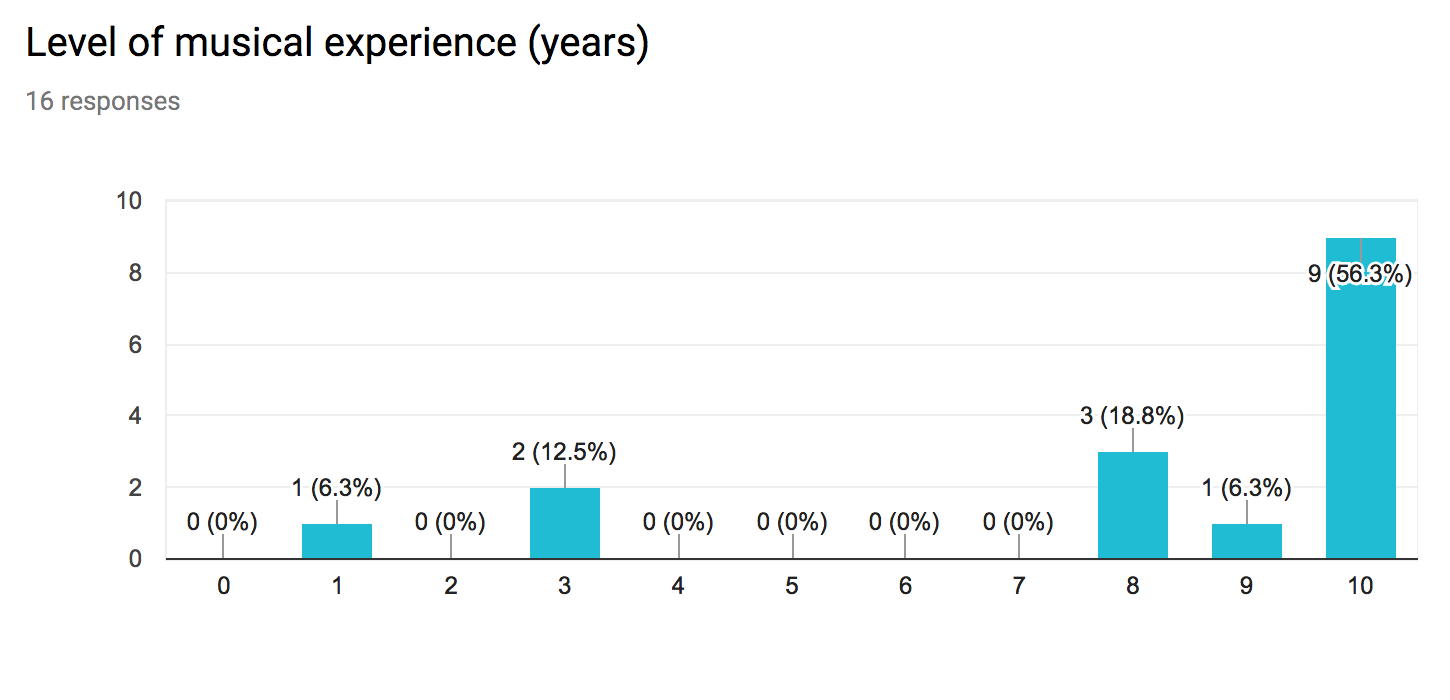
\includegraphics[width=\columnwidth]{musicExp}
    \caption{Musical Experience}
\end{figure}
The instrumental breakdown can be seen in Figure \ref{fig:pieInst} below.
\begin{figure}[H]\label{fig:pieInst}
    \centering
    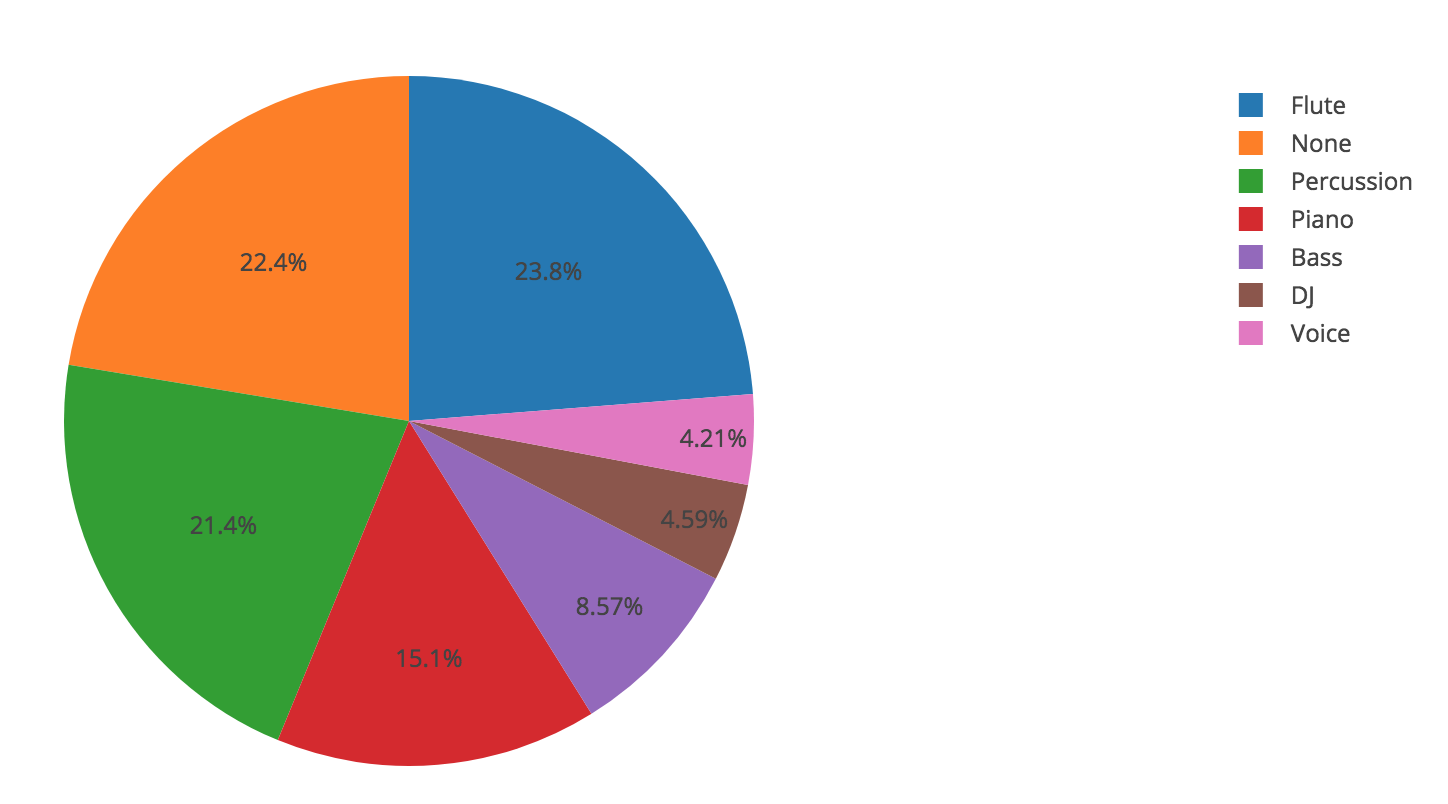
\includegraphics[width=\columnwidth]{pieInst}
    \caption{Spread of instrumental ability (out of 16)}
\end{figure}
Thirteen users had some sort of prior experience with an audible metronome and three did not. For most this was their first experience with a haptic device. All users chose their dominant arm to wear the haptic sleeve and chose their dominant hand for tapping.

\section{Results}
The main metric of stability and overall performance, as discussed in Section \ref{SMSTerms}, is the asynchrony. In all test cases a sanitization procedure was constructed to ensure that a missed tap would allow for the user to get back on track with the true onset later in the dataset - a process detailed entirely in Section \ref{sanitizationProcedure}. Finally, a latency correction factor was applied dependent on whether the test case was audible or haptic based. For more information on the derivation of this constant see Section \ref{latencyCalc}.

\subsection{SMS Research Expectations}
Prior SMS research has set expectations for the audible modality such that as the IOI increases the standard deviation of asynchrony $(SD_{asy})$ is expected to increase non linearly. This means that as we approach a slower bpm, we would anticipate larger deviations from the mean. This claim in in agreeance with the dataset across both modalities as shown in Figure \ref{fig:AllSummary} when viewing a subset of four test cases from right to left. For example, A3a1 relative to A3a4 and H1a1 compared to H1a4. These were test cases which had the highest inter-onset-interval and clearly exhibit high levels of variation relative to their adjacent test cases of higher bpm.
\begin{figure}[H]
    \centering
    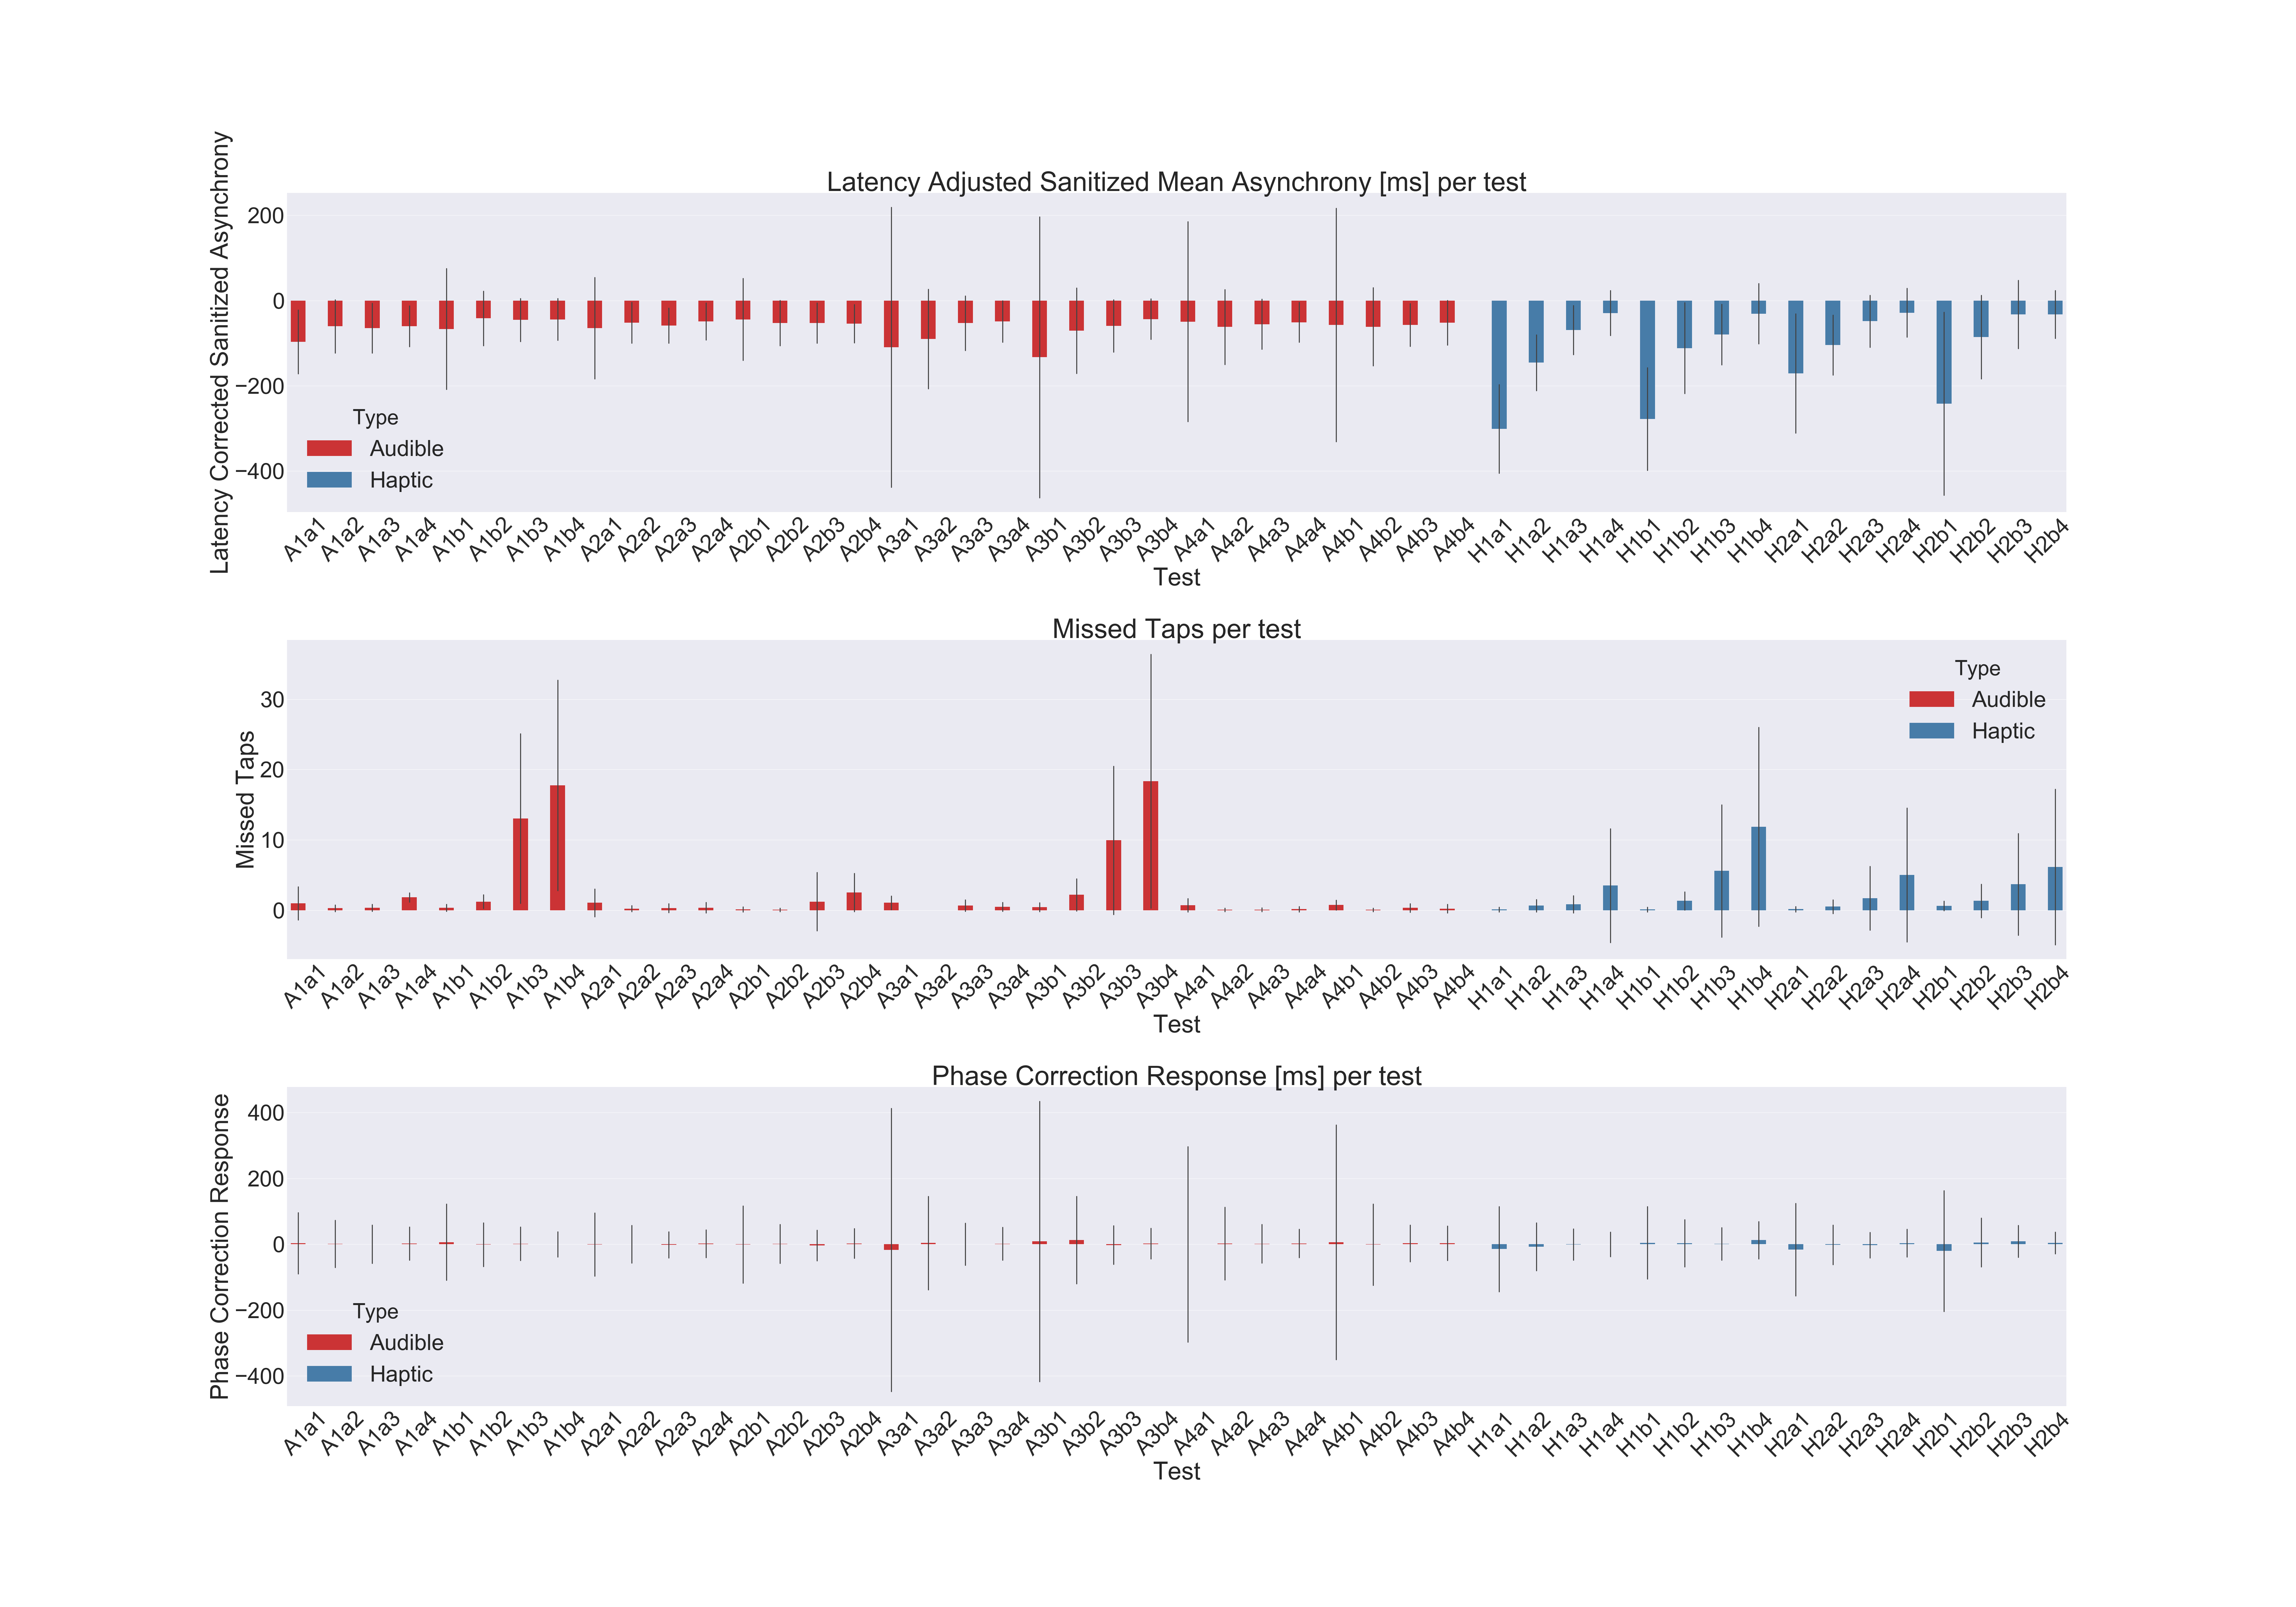
\includegraphics[width=\textwidth]{AllSummary}
    \caption{Summary across all participants}
    \label{fig:AllSummary}
\end{figure}

The black lines outline the standard deviation. The dynamic audible tests, A3a1 through A4b4, exhibited great deviation in both \textit{Latency Corrected Sanitized Asynchrony} (LCSA) and \textit{Phase Correction Response} (PCR), or the variation of one tap onset from the next.  The amount of metronomic jitter was varied on each repetition for these test cases and thus a reactionary response is expected since there was no real method of taking a proactive approach for these particular tests.

Most taps were missed during the interstitial legato chime or swing click A1b3, A1b4, A3b3, A3b4 as well as during the ramp up haptic test cases H1b3 and H1b4. These test cases ranged from 120 bpm to 180 implying either an indistinct onset, overstimulation, or low signal to noise ratio.

SMS research expects a trend towards positive mean asynchrony when approaching the biomechanical limit (<300 ms or 180 bpm)


This claim is in partial agreement with the results found in Figure \ref{fig:sLCSAvIOI}. There is a trend within the static audible test cases which break linearity at two points, once around 325 and again just before 700. These equate to an bpm level between 85 and 185. 

\subsubsection{Group Trends}
SMS findings anticipate a lower $(SD_{asy})$ for professionals compared to non musicians and expect little to no difference between amateurs and non musicians. As seen in Figure \ref{fig:GroupSummaries}, the results agree with past research. Professionals had a mean LCSA of approximately -45 ms across all audible tests and approximately -75 ms for haptic tests relative to -55 and -90 ms for amateurs and -90 and -80 ms for non-musicians.

The non-professional group did marginally better on the haptic test cases than audible, though with a higher amount of missed taps. The standard deviation of the phase correction response, shown at the bottom of the figure, implies an ability to adapt tapping synchronization from beat to beat more successfully with the haptic device than across audible tests. This lends very promising insight but must be further classified to determine if the benefit is test case dependent or involving of strictly non-isochronous beats.
\begin{figure}[H]
    \centering
    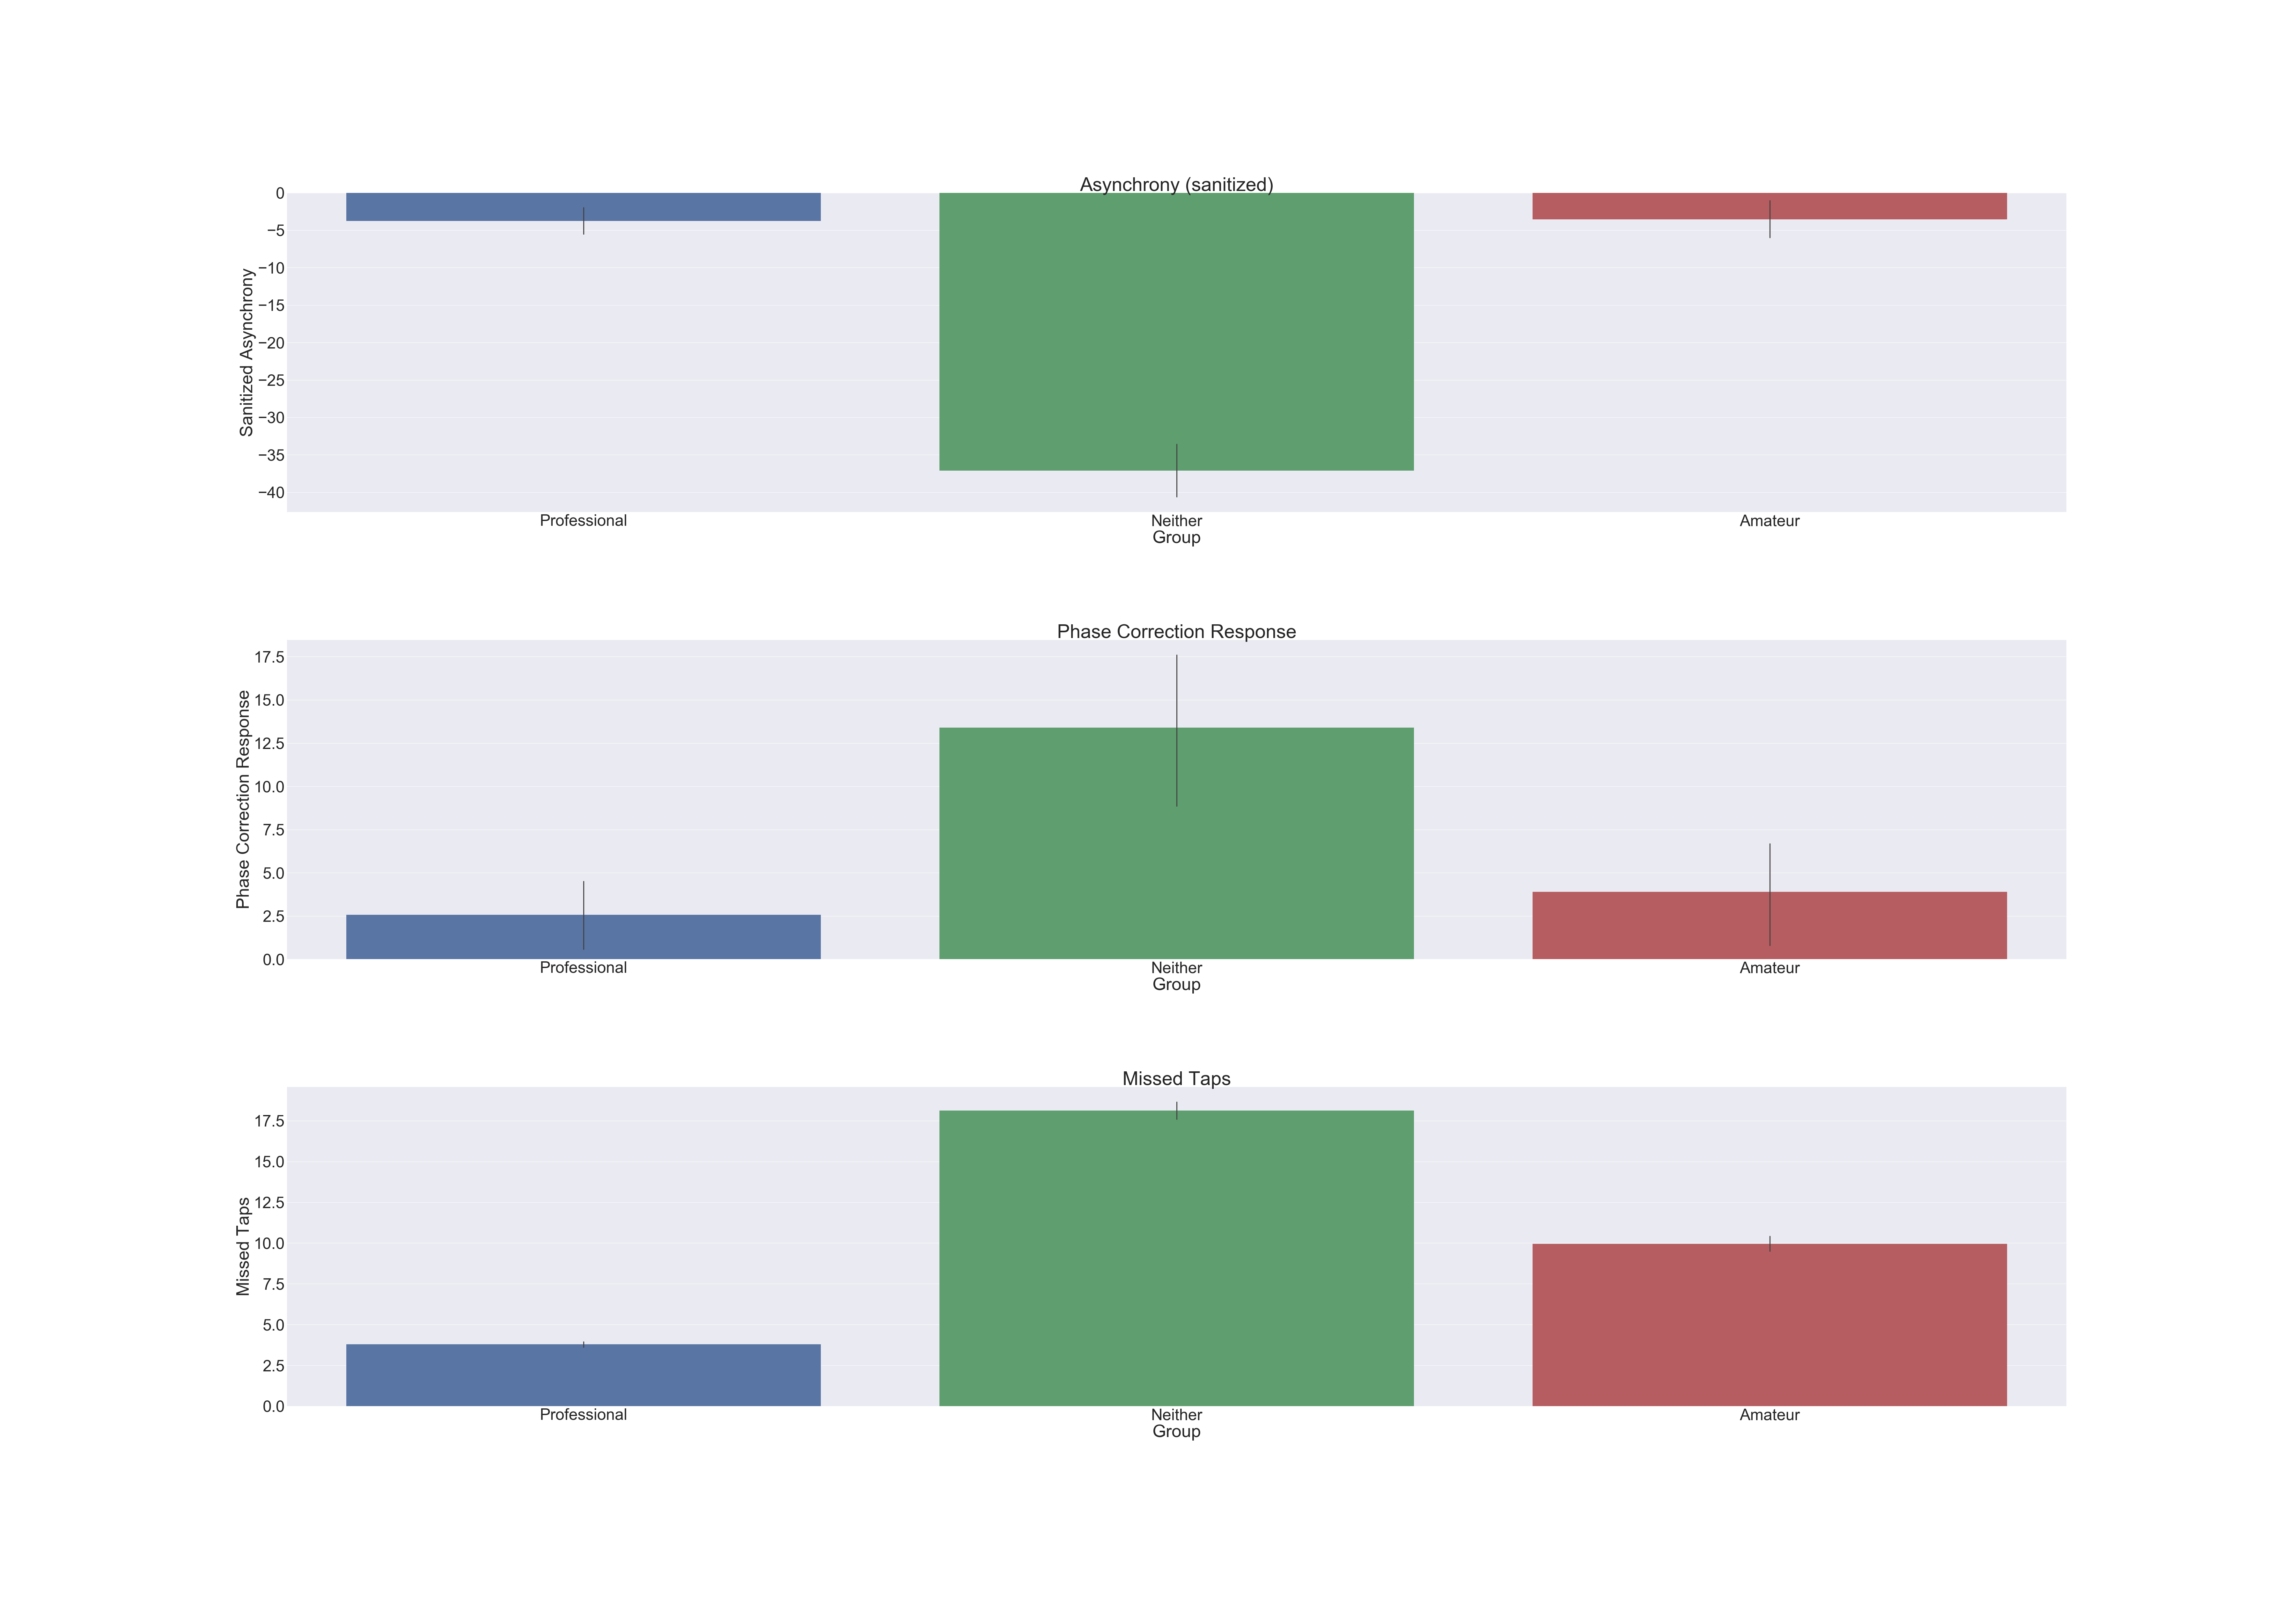
\includegraphics[width=\textwidth]{GroupSummaries}
    \caption{Group test summaries}
    \label{fig:GroupSummaries}
\end{figure}
\subsection{Instrumental Breakdown}

Past research into sensorimotor synchronization suggests a heightened rhythmic sensibility within percussionists and pianists who notoriously have held lowest variability values for tap tests. Figure \ref{fig:InstrumentSummaries} would suggest agreeance with the exception of Bass yet the bins are uneven. For instance, whereas there was only a single bassist in the test, there were four percussionists.

\begin{figure}[H]
    \centering
    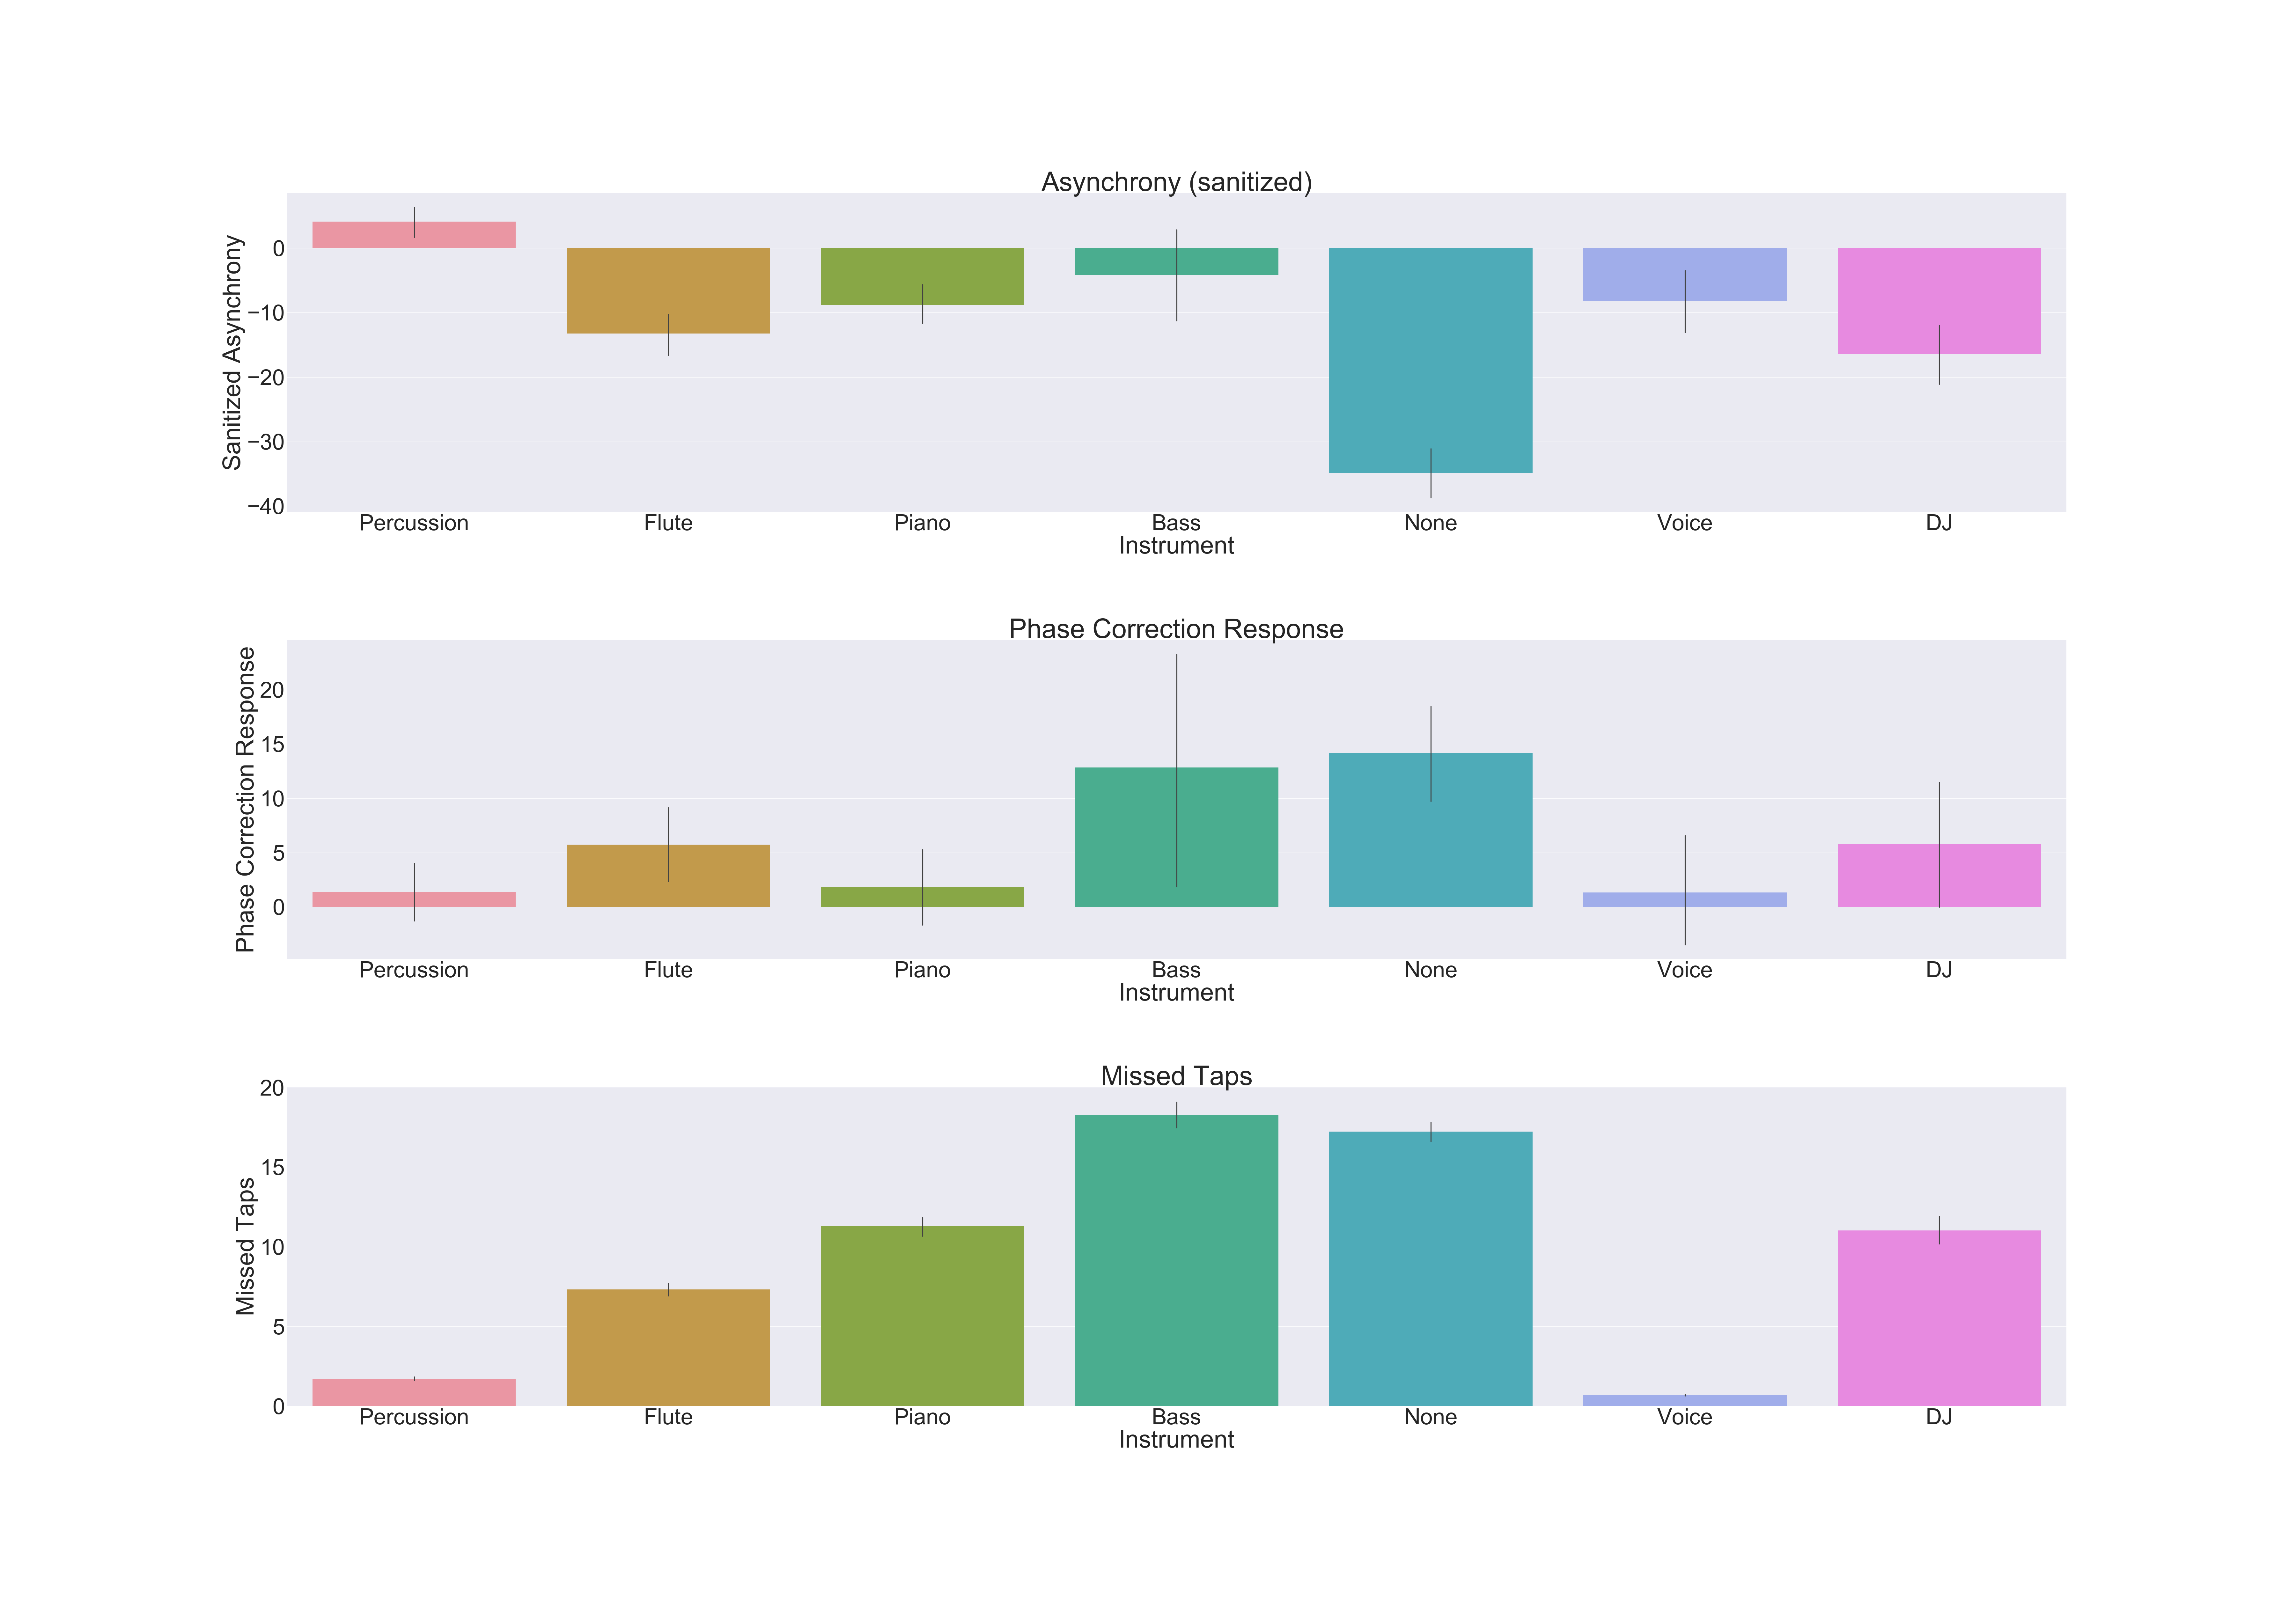
\includegraphics[width=\textwidth]{InstrumentSummaries}
    \caption{Summaries per instrument}
    \label{fig:InstrumentSummaries}
\end{figure}

\section{Haptic Dynamic Tests}
In a breakdown of asynchrony for static versus dynamic tests per group as shown in Figure \ref{fig:fig:LCSA_KDE}, the dynamic haptic test cases exhibit a shift towards zero which implies an improvement in synchronization during non-isochronous beats. 
\begin{figure}[H]
    \centering
    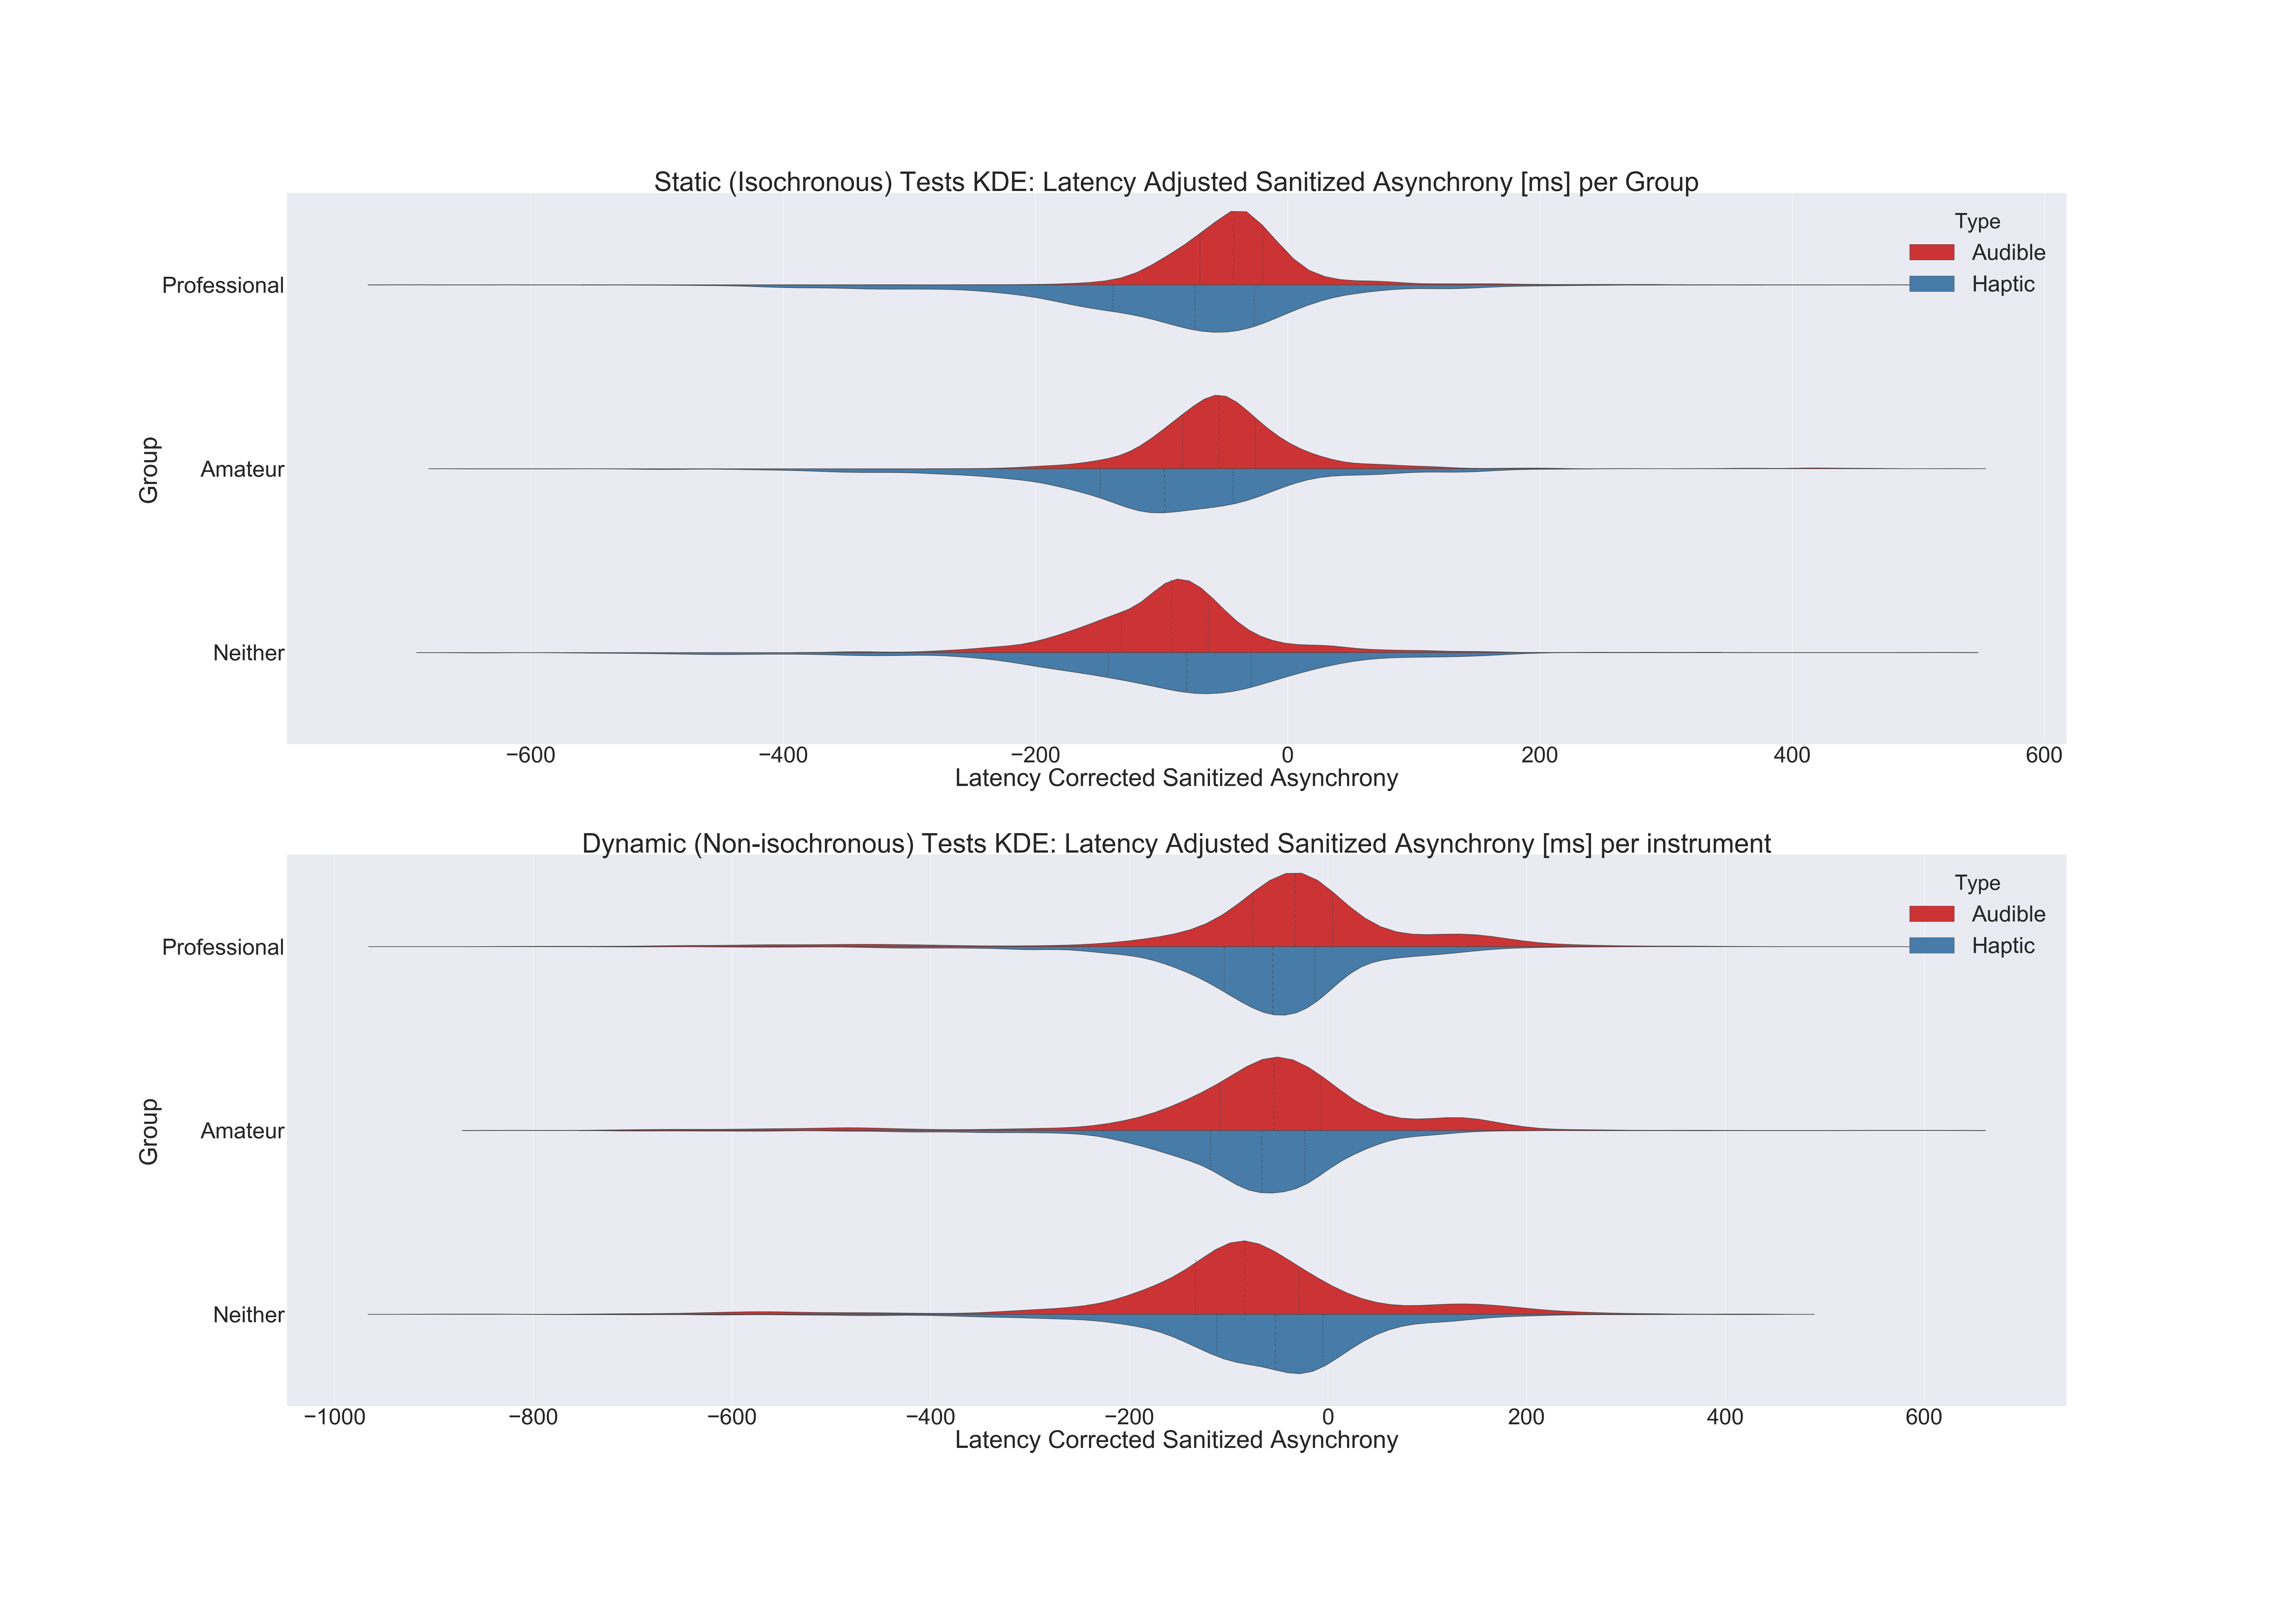
\includegraphics[width=\textwidth]{LCSA_KDE}
    \caption{Kernel Density Estimation: Latency Corrected Sanitized Asynchrony for Static vs Dynamic Tests}
    \label{fig:LCSA_KDE}
\end{figure}

This finding heavily supports the overarching hypothesis of this work and can be further exemplified in Figure \ref{fig:sLCSAvIOI} and \ref{fig:dLCSAvIOI} below. As we traverse from left ot right on the graph, the IOI increases and therefore represents a decreasing bpm. The trajectory is nearly flat for the static audible test cases in red at the top. 

\begin{figure}[H]
    \centering
    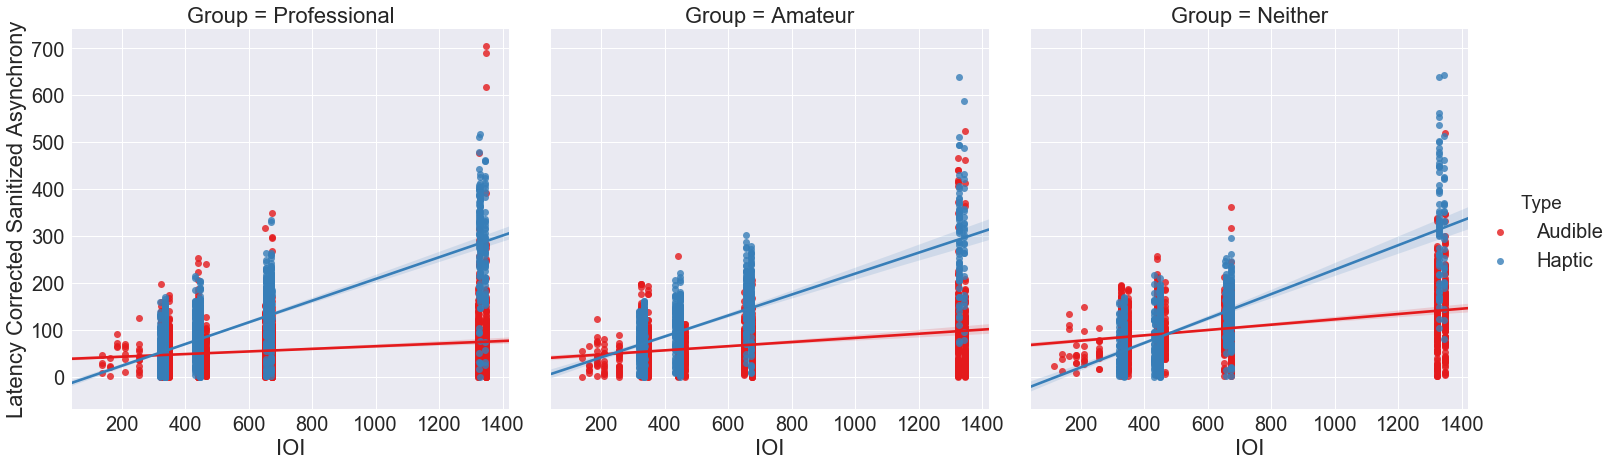
\includegraphics[width=\textwidth]{steady_LCSA_vs_IOI}
    \caption{Latency Corrected Sanitized Asynchrony vs. Inter-Onset-Interval across static test cases.}
    \label{fig:sLCSAvIOI}
\end{figure}

The dynamic audible tests trend towards a positive asynchrony implying a reactive approach. The haptic tests contrarily trend steeply toward negative asynchronies for both static and dynamic test cases, the deviation implies a proactive approach. Overall, the users were concretely able to navigate non-isochronous beats successfully in a pre-emptive fashion with the haptic metronome device. 
\begin{figure}[H]
    \centering
    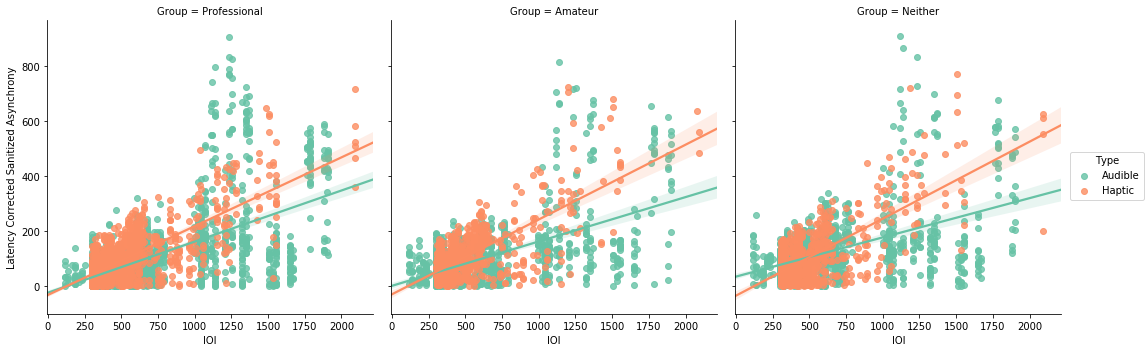
\includegraphics[width=\textwidth]{dynamic_LCSA_vs_IOI}
    \caption{Latency Corrected Sanitized Asynchrony vs. Inter-Onset-Interval across dynamic test cases.}
    \label{fig:dLCSAvIOI}
\end{figure}

\subsection{Analysis of variance across test cases}

To confirm the significance of difference between haptic and audible tests, an independent t-test with unequal variance was conducted. The null hypothesis was the assumption of no difference between these test case types in the latency corrected sanitized asynchrony value. P-values were obtained for haptic versus audible test case combinations across the static and dynamic groupings. The results are summarized in Figure \ref{pvalue}.

\begin{figure}[H]
    \centering
    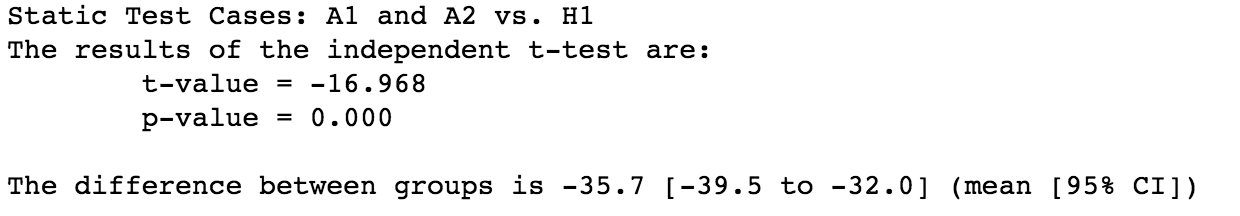
\includegraphics[width=\textwidth]{StaticP}
    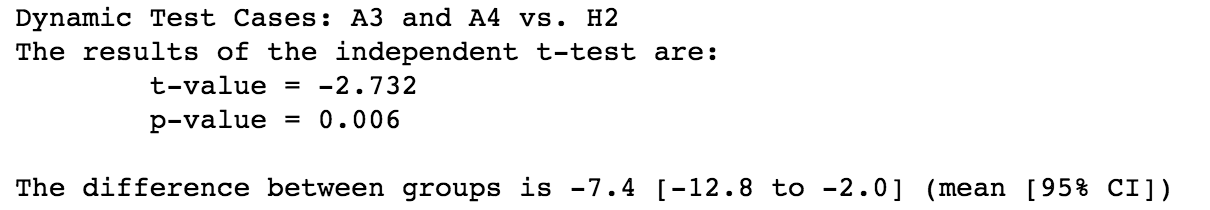
\includegraphics[width=\textwidth]{DynamicP}
    \caption{T-Test Results}
    \label{fig:pvalue}
\end{figure}

\section{Feedback}
On a scale of 1 to 10, with 10 being the most difficult, approximately 70\% of those tested found synchronization to the steady audible beat to be a level of 1, or extremely easy. The remaining 30\% found it to be either a 2 or 4 level of difficulty. However, the spread for dynamic audio test cases was wide ranging with the majority expressing a high level of difficulty 81.3\% above level 5 seen in Figure \ref{fig:Auddiff}.

\begin{figure}[H]
    \centering
    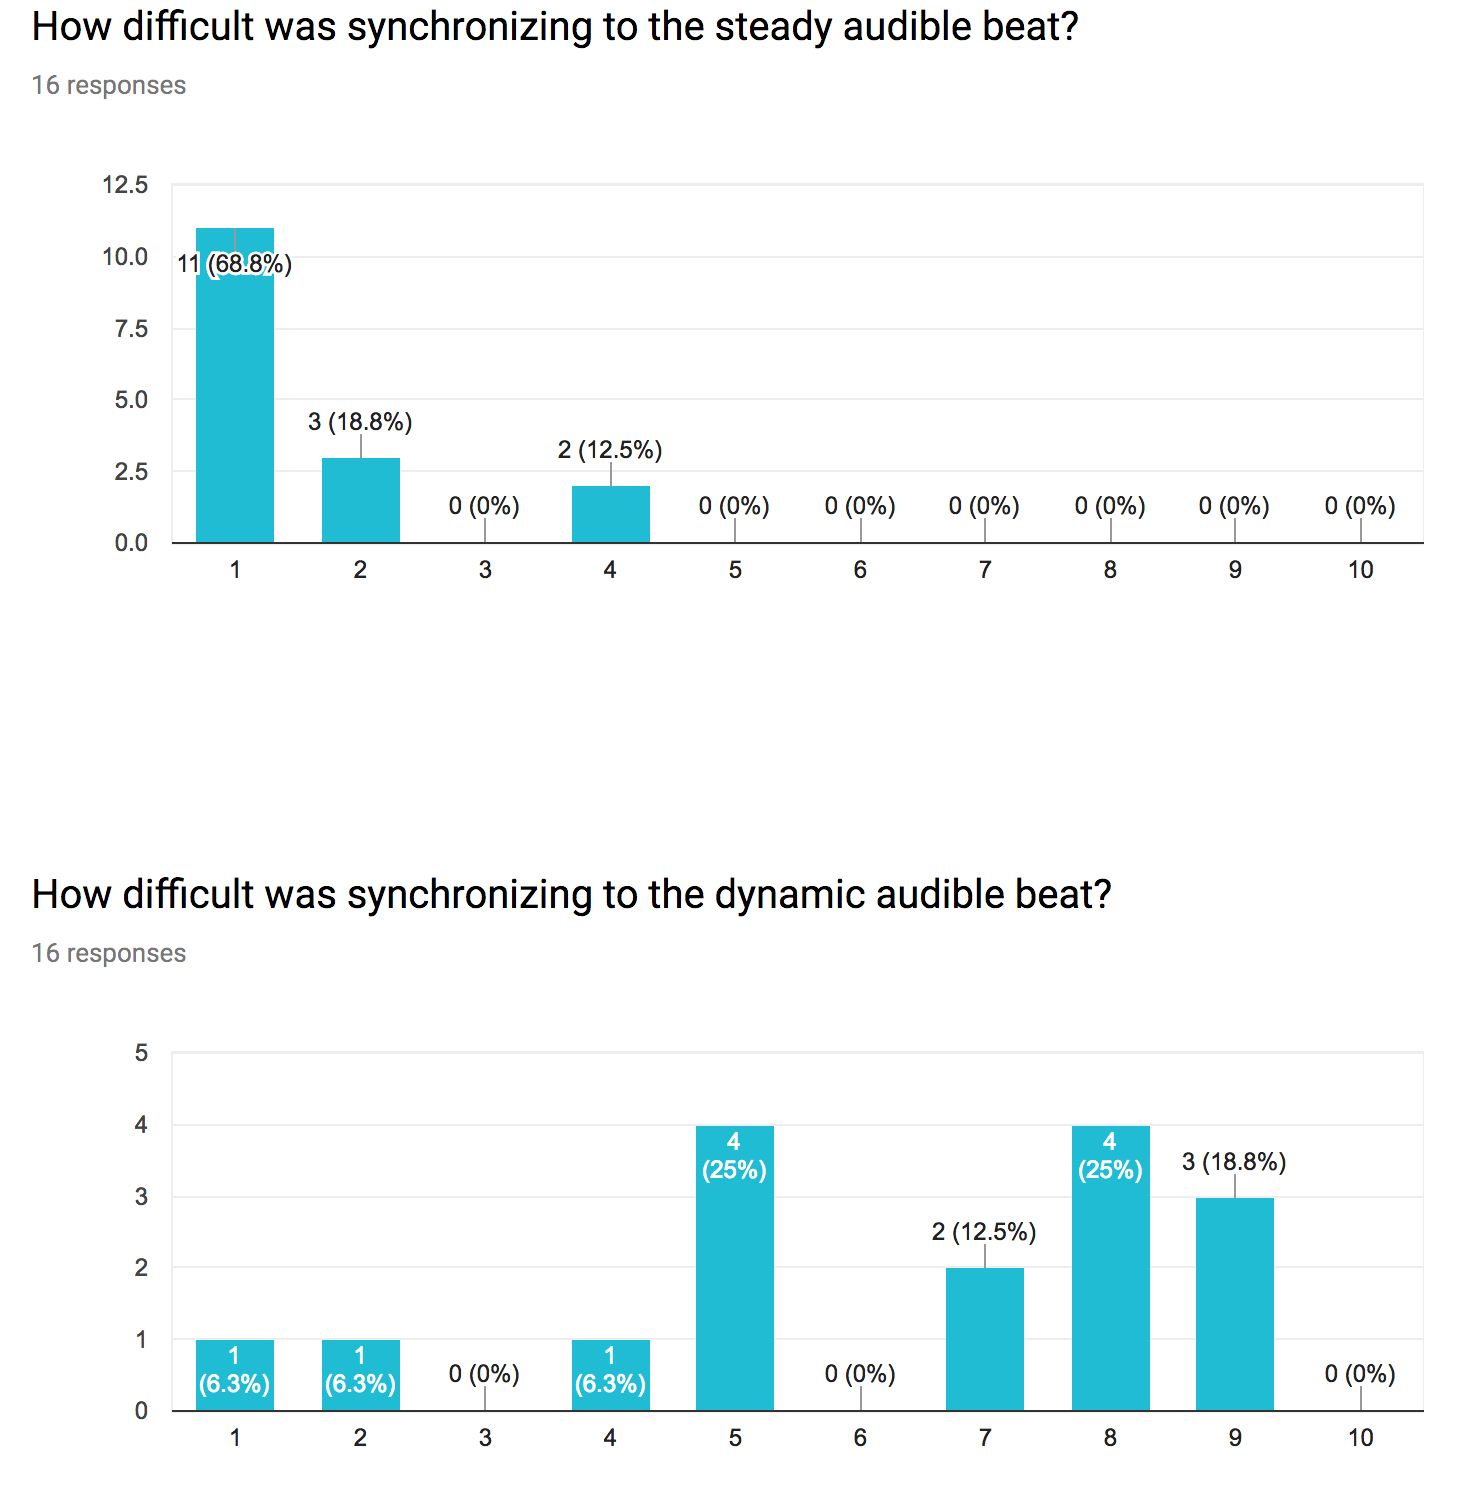
\includegraphics[width=\columnwidth]{Auddiff}
    \caption{Questionnaire: Difficulty results for dynamic audible tests.}
    \label{fig:Auddiff}
\end{figure}

The haptic tests had a wider difficulty spread across the steady beat shown at the top of Figure \ref{fig:Hapdiff}. This was to be expected as users had no prior experience with this haptic device let alone any other sort of wearable metronome. If retested or trained over the course of a few weeks to the sensation of touch the responses might have been more favorable or closer in resemblance to the static audible tests. Regardless, the dynamic beat for the haptic modality yielded less difficulty rankings than the dynamic audible (11 ranked a level of 5 or more difficulty vs. 13 for audible dynamic tests), which further supports the hypothesis of this work.
\begin{figure}[H]
    \centering
    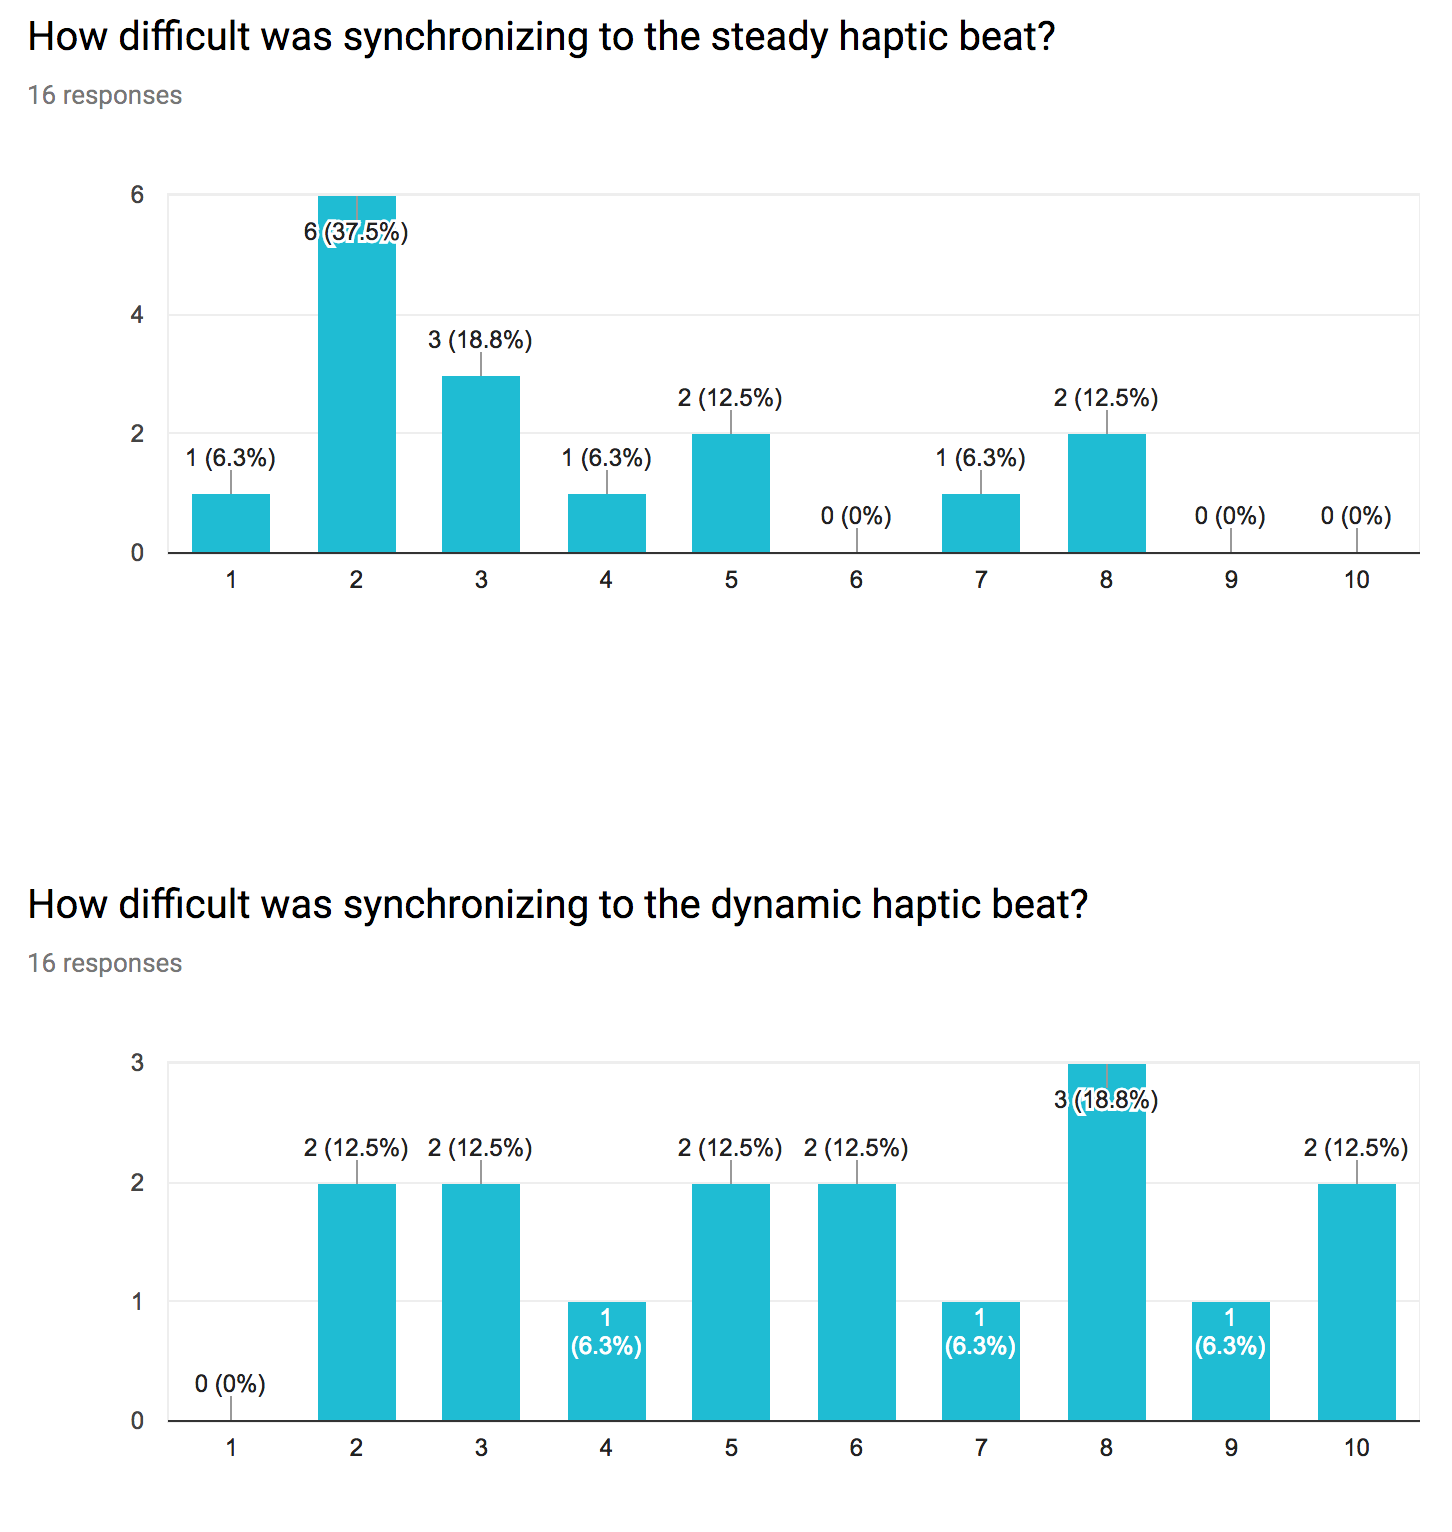
\includegraphics[width=\columnwidth]{Hapdiff}
    \caption{Questionnaire: Difficulty results for dynamic haptic tests.}
    \label{fig:Hapdiff}
\end{figure}

With the question of modality preference, auditory won hands down for the steady beat. Some users would have preferred a combination of both auditory and haptic, though the option was not exemplified throughout in the test suite. The haptic won by 13\% for the dynamic tests, shown in Figure \ref{fig:modPref}
\begin{figure}[H]
    \centering
    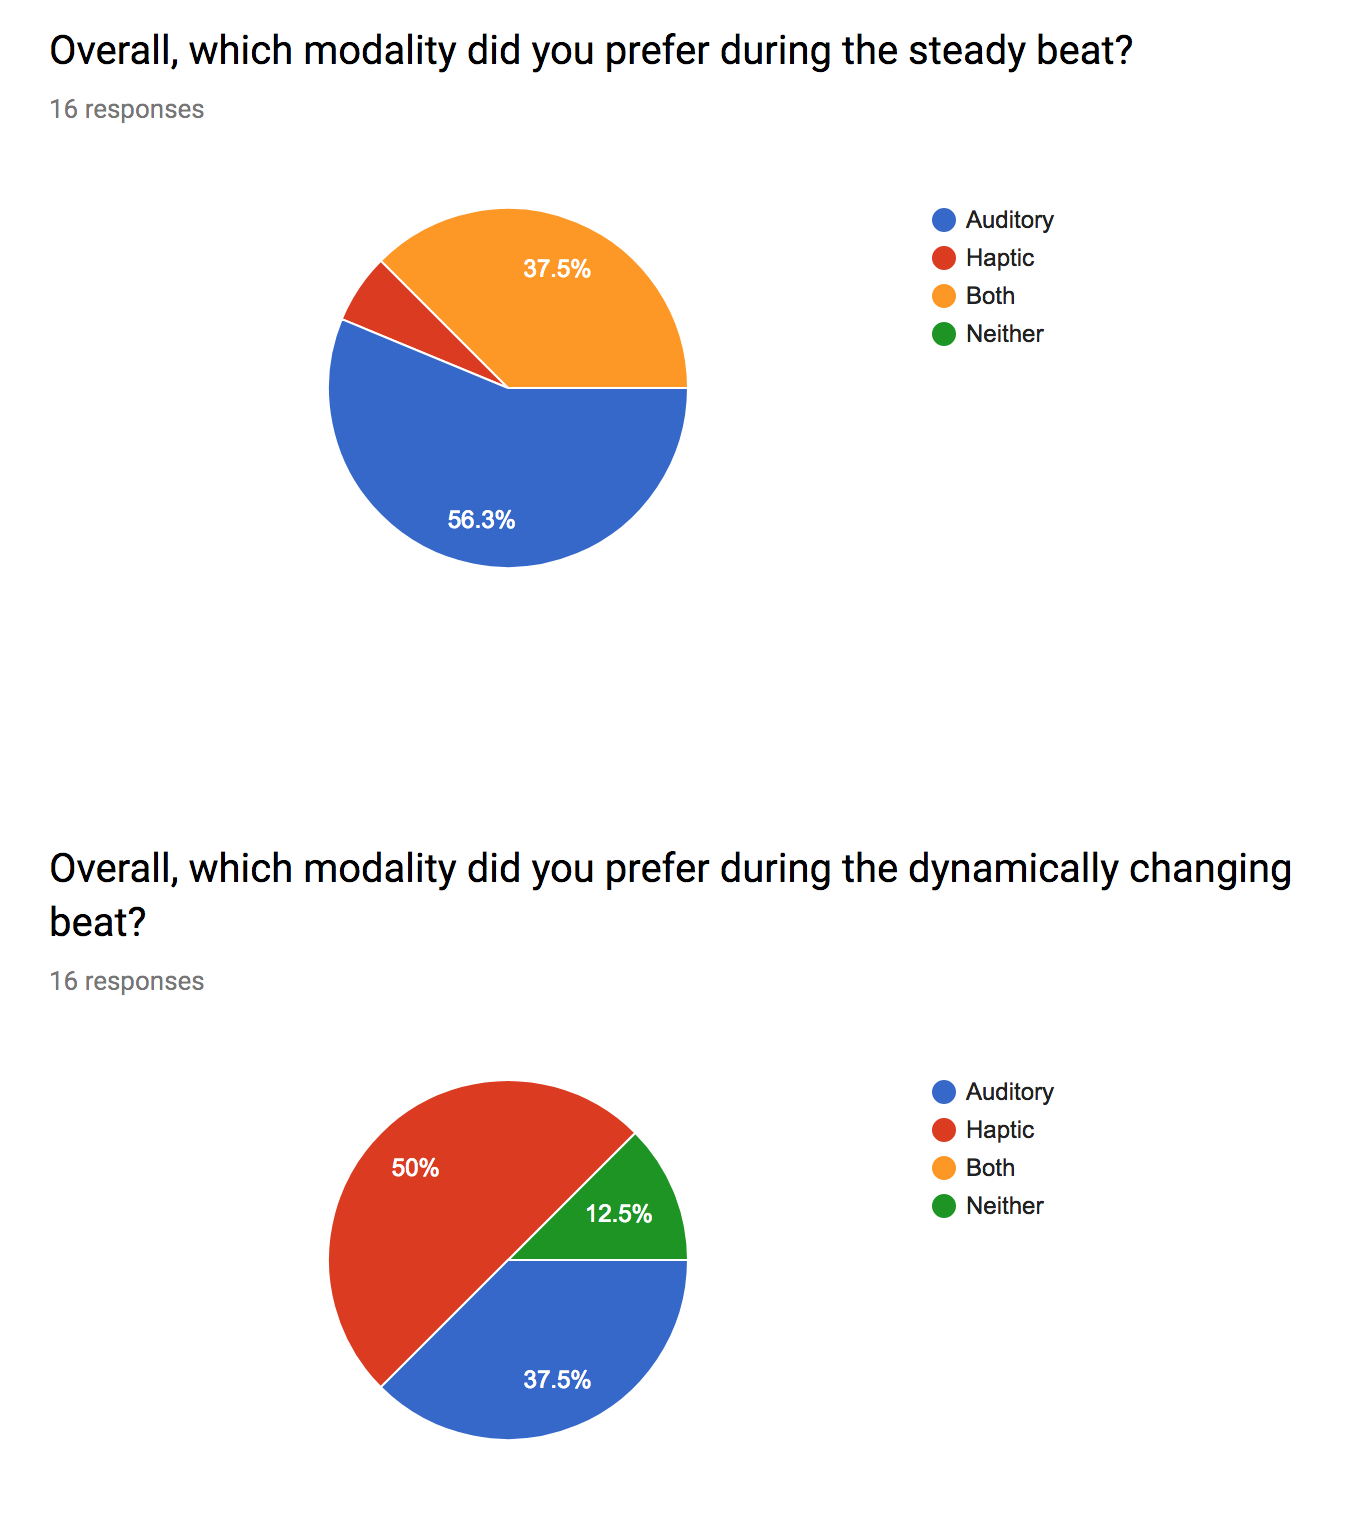
\includegraphics[width=\columnwidth]{modPref}
    \caption{Questionnaire: Modality preference}
    \label{fig:modPref}
\end{figure}

When asked specifically about the preference for haptic mode of operation, it seemed that most users preferred the all on all off mode see in Figure \ref{fig:hspace}
\begin{figure}[H]
    \centering
    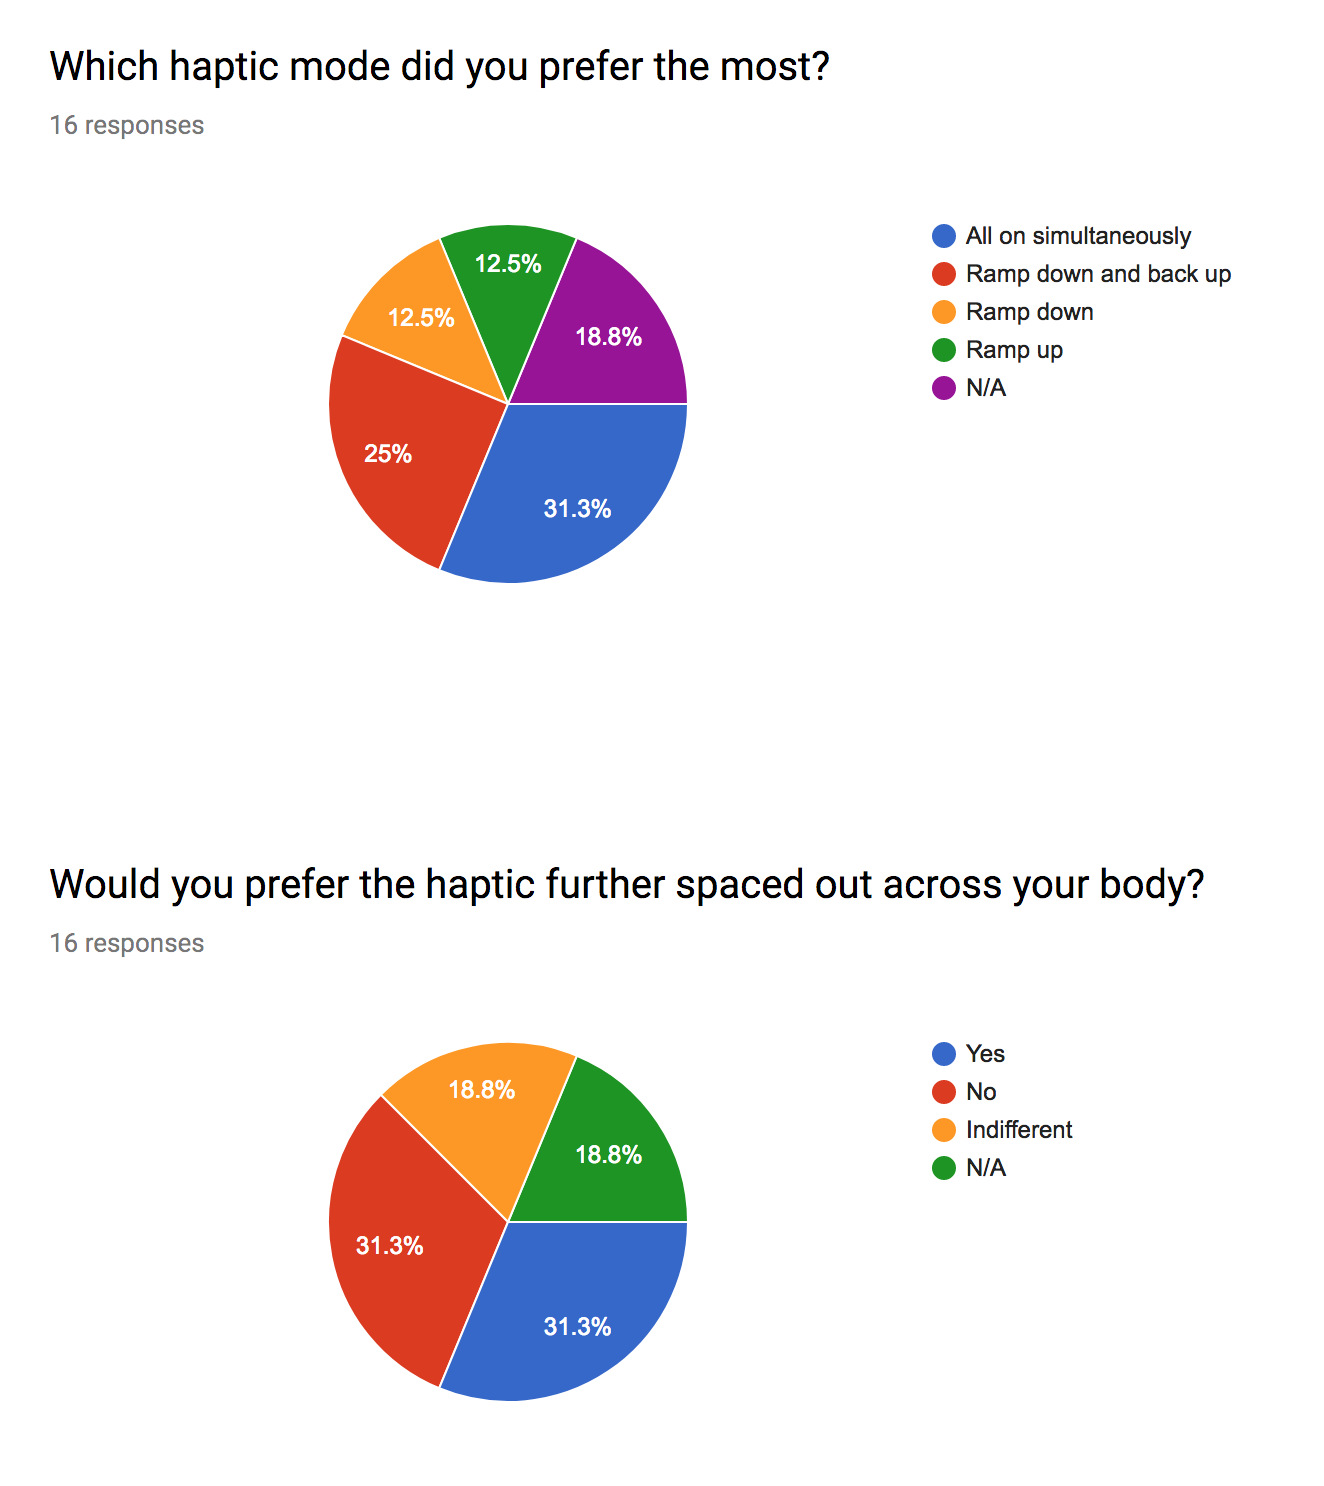
\includegraphics[width=\columnwidth]{hspace}
    \caption{Questionnaire: Haptic mode preference and spacing}
    \label{fig:hspace}
\end{figure}

This could be attributed to the lack of stimulation strength at higher vibrating frequencies for the ramping mode, an intrinsic flaw due to the nature of power operation of the haptic prototype at 5 V 500 mA laptop USB max output - remedied with the battery-dependent next design iteration discussed in Chapter \ref{wirelessHP}. 

Furthermore, the users were tested at up to (and occasionally past) 180. This is well beyond the documented 150 bpm limit. At such rapid speeds the vibrotactiles had little time to ramp up to full capacity. This was another reason for diminished strength and yielded a sensation indistinguishable from noise.

When asked about placement preference, there was a 31.3\% split between the desire to have it further spaced or not. Prior research advocates a larger area of coverage to isolation stimulation zones and therefore promote perceptivity. This would be adopted in a more flexible way on the next prototype iteration with velco straps that can be spaced out however desired.

\section{Conclusions}
Overall, the results are quantitatively promising in support of the hypothesis that filling in the interstitial space provides benefit for non-isochronous or dynamic beats.

\begin{figure} \label{fig:BoxPlotSvD}
    \centering
    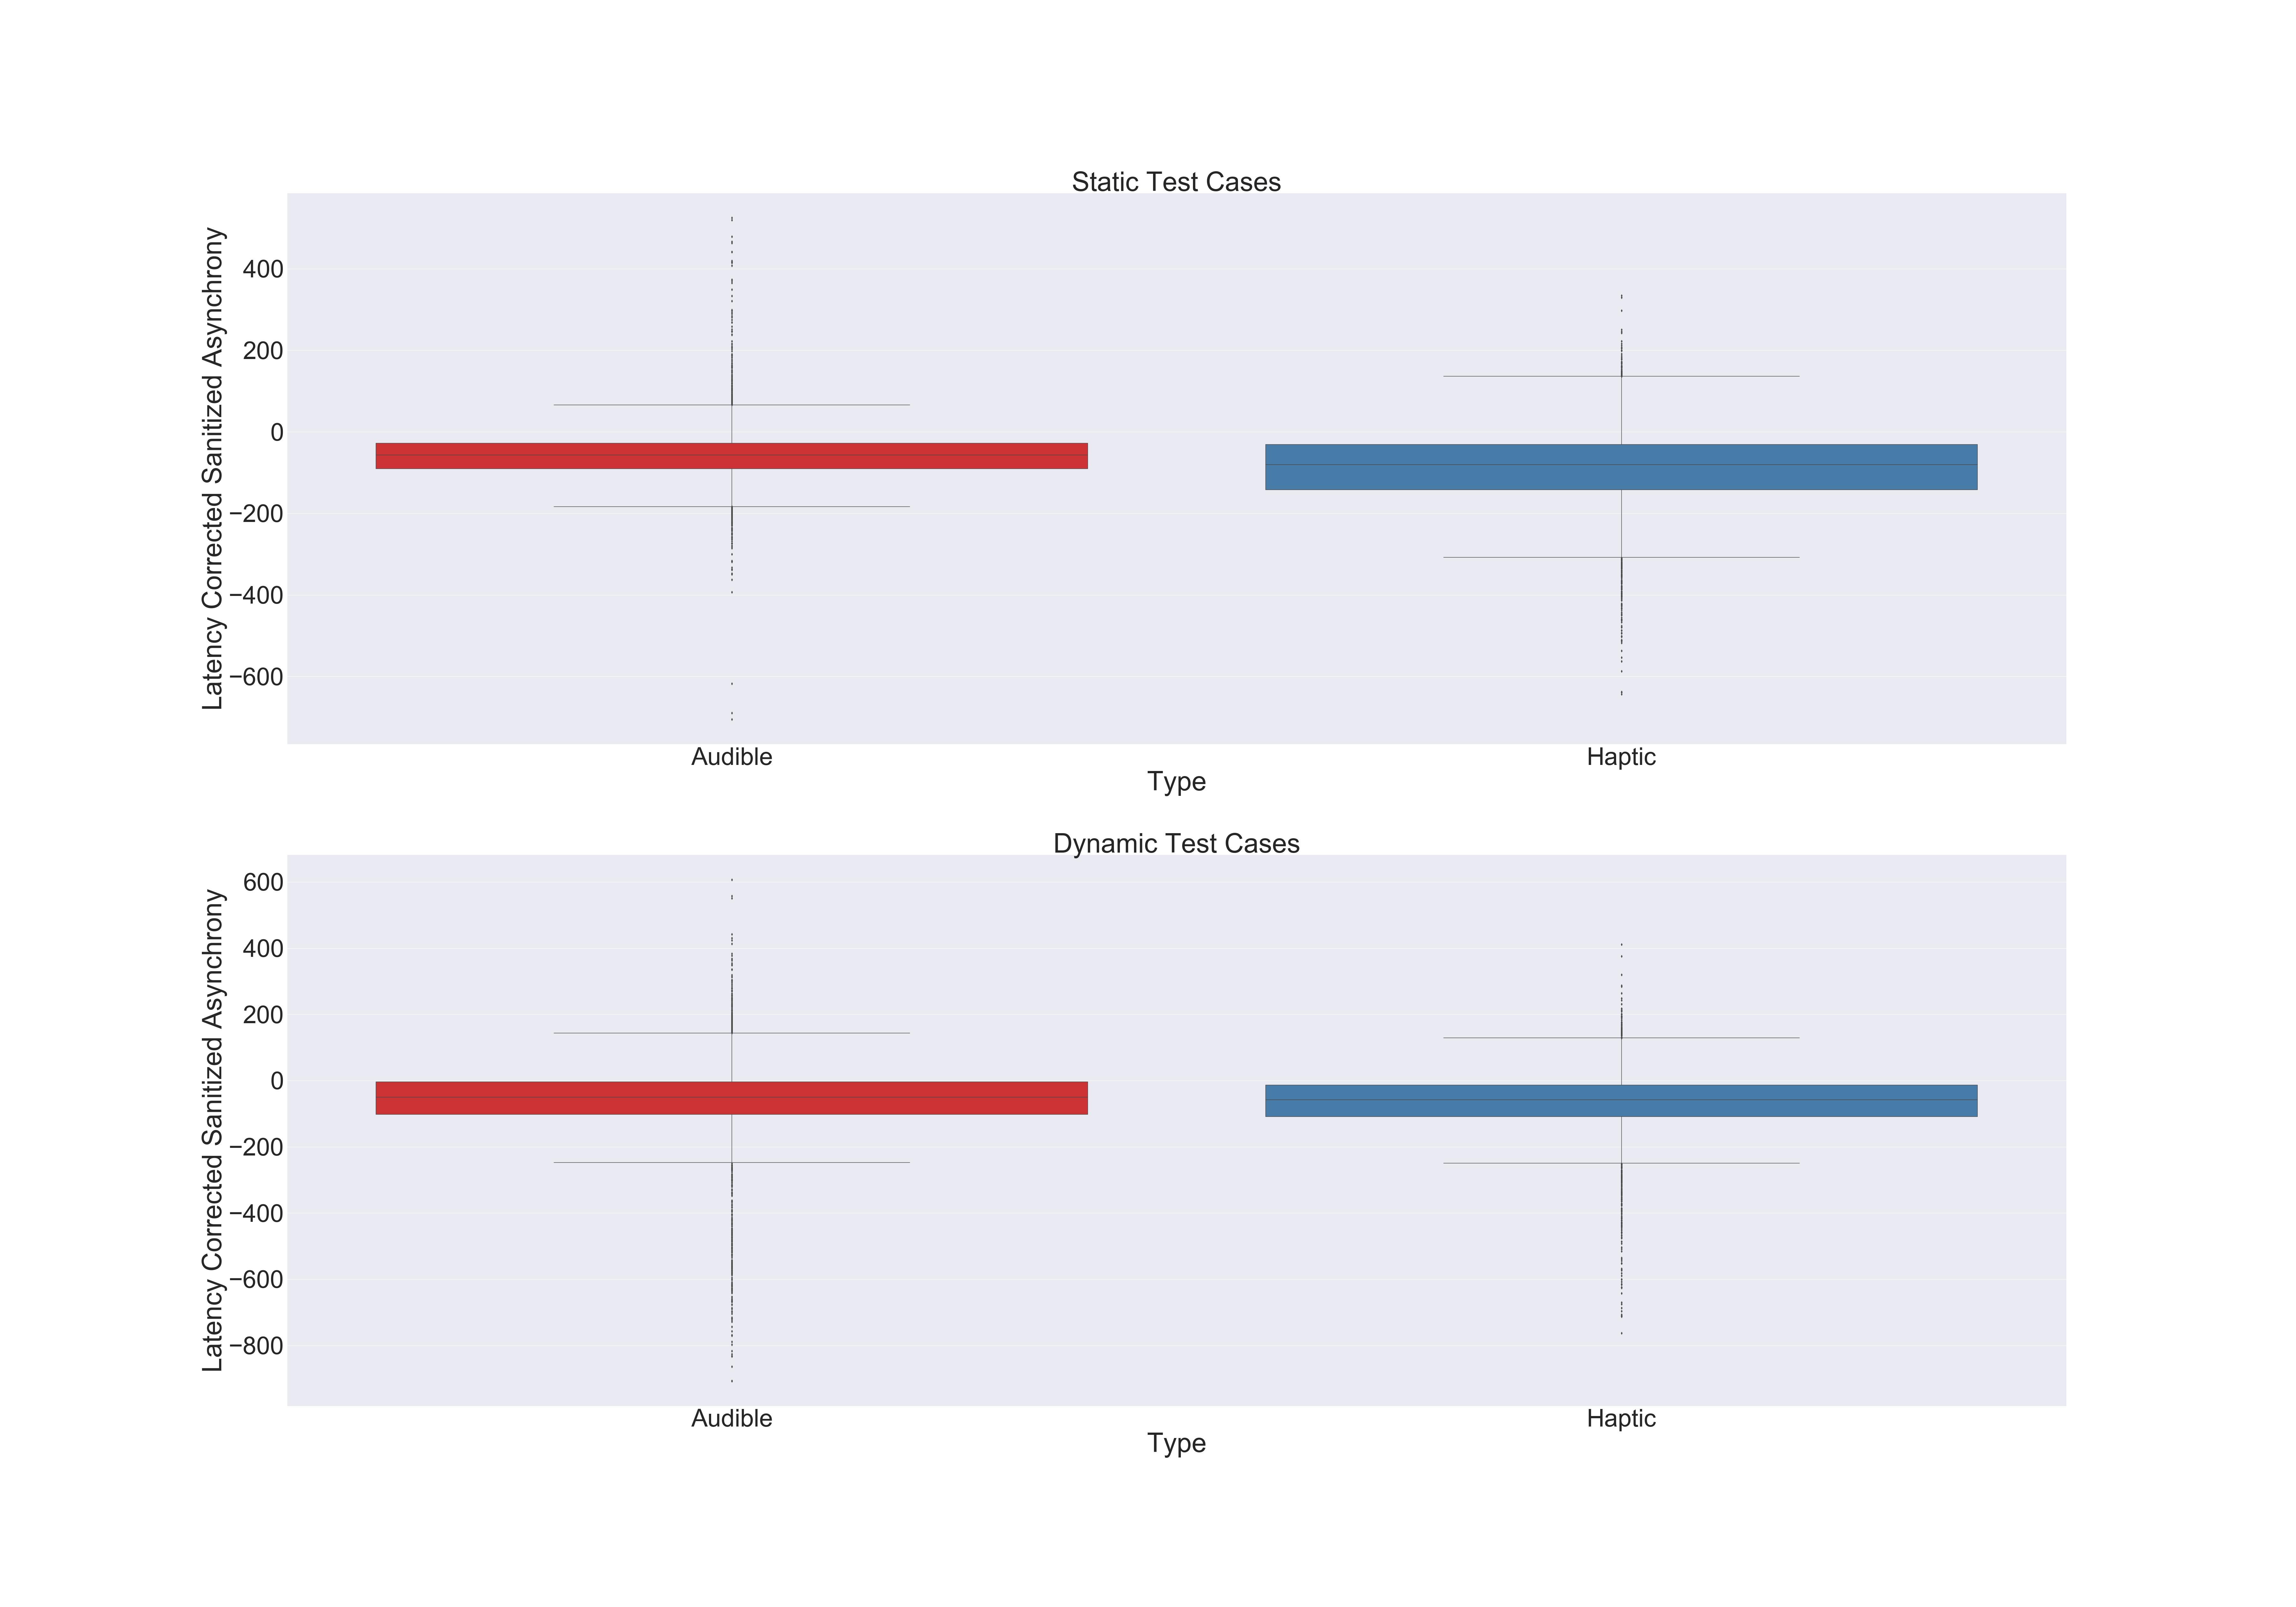
\includegraphics[width=\columnwidth]{BoxPlotSvD}
    \caption{Box plot overall results: Static above, haptic below}
\end{figure}